\chapter{Genetic structure of human populations in Great Britain}

As we've seen several times in this course, the amount of genetic data
available on humans is vastly greater than what is available for any
other organism. As a result, it's possible to use these data to gain
unusually deep insight into the recent history of many human
populations. Today's example comes from Great Britain, courtesy of a
very large consortium~\cite{Leslie-etal-2015}

\section*{Data}

\begin{itemize}

\item 2039 individuals with four grandparents born within 80km of one
  another, effectively studying alleles sampled from grandparents
  (ca. 1885). 

\item 6209 samples from 10 countries in continental Europe.

\item Autosomal SNPs genotyped in both samples~(ca. 500K). 

\end{itemize}

\section*{Results*}

Very little evidence of population structure within British sample

\begin{itemize}

\item Average pairwise $F_{ST}$: 0.0007

\item Maximum pairwise $F_{ST}$: 0.003

\end{itemize}

Individual assignment analysis of genotypes using {\tt
  fineSTRUCTURE}. Same principle as {\tt STRUCTURE}, but it models the
correlations among SNPs resulting from gametic disequilibrium, rather
than treating each locus as being independently inherited. The
analysis is on {\it haplotypes\/} rather than on alleles. In addition,
it clusters populations
hierarchically~(Figure~\ref{fig:fine-structure}\index{fineSTRUCTURE}\index{human
  population genetics}

\begin{figure}
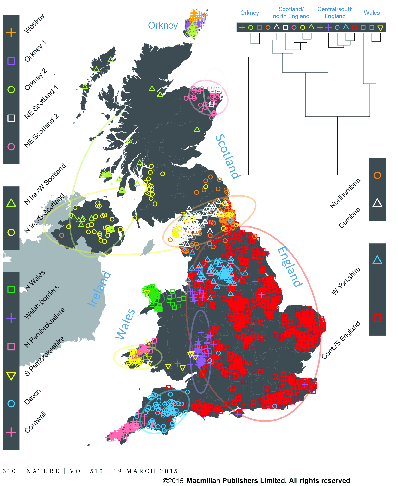
\includegraphics[height=0.9\textheight]{fine-structure-britain.eps}
\caption{{\tt fineSTRUCTURE} analysis of genotypes from Great Britain~(from~\cite{Leslie-etal-2015}).}
\end{figure}

Analysis of the European data identifies 52 groups. The authors used
{\tt Chromopainter} to construct each of the haplotypes detected in
their sample of 2039 individuals from the UK as a mosaic of haplotypes
derived from those found in their sample of 6209 individuals from
continental Europe. Since they know (a) the UK cluster to which each
UK individual belongs and (b) the European group from which each
individual contributing to the UK mosaic belongs they can estimate (c)
the proportion of ancestry for each UK cluster derived from each
European group. The results are shown in Figure~\ref{fig:UK-Europe}

\begin{figure}
\begin{center}
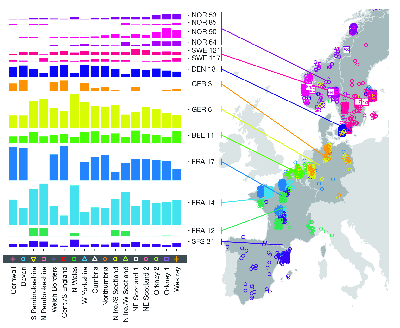
\includegraphics[width=0.9\textwidth]{UK-Europe.eps}
\end{center}
\caption{European ancestry of the 17 clusters identified in the UK~(from~\cite{Leslie-etal-2015}).}\label{fig:UK-Europe}
\end{figure}

